\subsection{Appearance of new words}

We consider the rate at which new 1-grams are incorporated in the vocabulary, and the nature of those words,  as a crucial component of linguistic drifts. It was thus important to come up with a reliable way to quantify this process .\\

A simple approach to estimate the apparition of new words would be to sum up the number of distinct 1-grams for each year and then monitor its evolution. But this suffers several drawbacks : first the remaining OCR errors, that still account for a substantial portion of the distinct 1-grams,  would be incorrectly considered as emerging words.  Furthermore, it would not provide any clue about the actual amount of words entering/exiting the set of used words, but only snapshots of how many words are in fashion at any point in time. Those two aspects would in our opinion have strongly distorted the resulting figures, this is why we opted for a different procedure.\\

The ideas was to define a pair of thresholds, one below which a word would be considered as not existing and a higher one meaning that the 1-gram is commonly used. The lower bound is not zero such as to take possible OCR correction into account. Once the higher threshold has been crossed, we require the frequencies to stay above the threshold R\% of the time.  This filter will only detect words that appear quite suddenly and as the advantage that we can determine the precise time where the words appeared (inferred from \textit{zerosSeqAtStart}). Figure \ref{algoschema} is meant to illustrate the algorithm.\\

\begin{figure}[h!]
        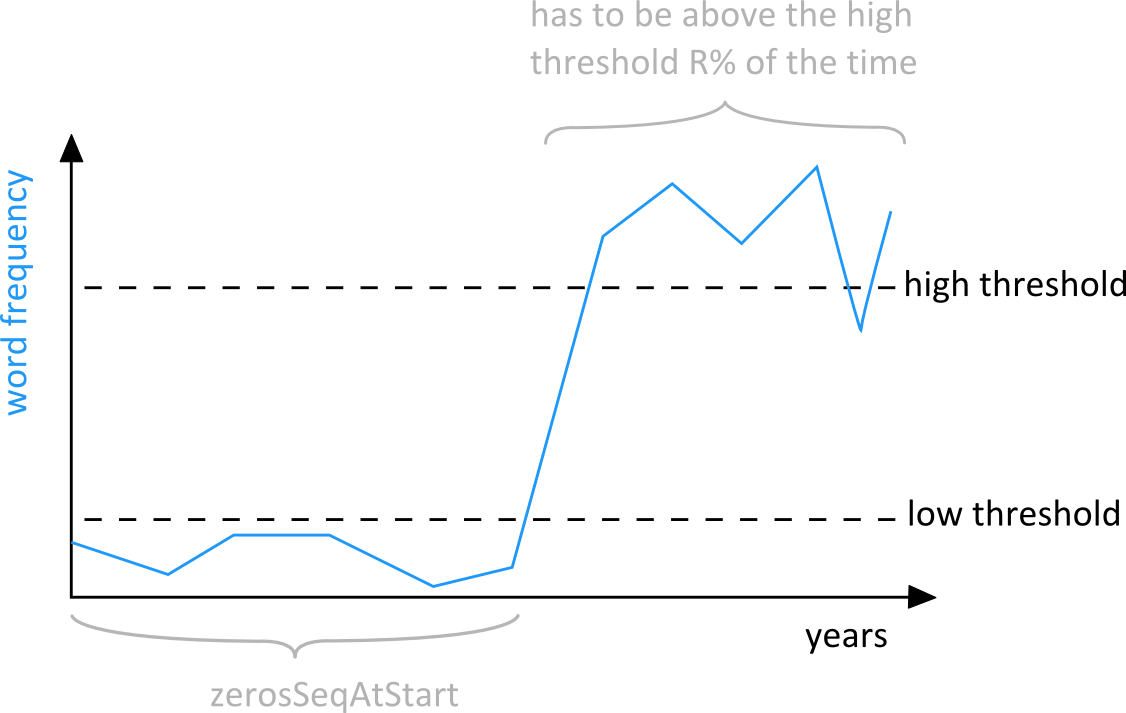
\includegraphics[scale=0.7]{Pictures/statistics/appearing-words/algo-schema.png}
        \caption{Visualization of the detection algorithm's behavior}
        \label{algoschema}
	\centering
\end{figure}

Figures \ref{ratio60} and \ref{ratio80} show the amounts of words spotted as appearing, using frequencies averaged over range of 5 years.  In our opinion the results for the first 15 year are overly influenced by the fact that they contains very few articles compared to other years (factor of 6). We see a clear increase in term of world creation recently, no matter the set of parameters selected. 
\begin{figure}[h!]
        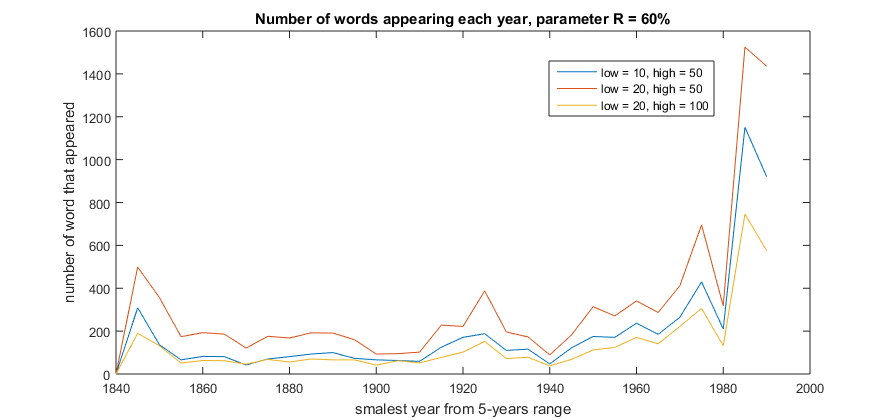
\includegraphics[scale=0.65]{Pictures/statistics/appearing-words/word-appearing-ratio60.png}
        \caption{New words detection with tolerance rate R = 60\%}
        \label{ratio60}
	\centering
\end{figure}
\begin{figure}[h!]
        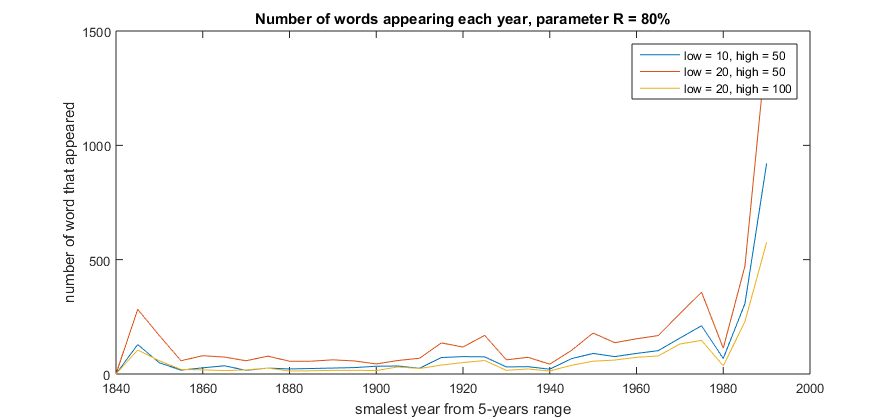
\includegraphics[scale=0.65]{Pictures/statistics/appearing-words/word-appearing-ratio80.png}
        \caption{New words detection with tolerance rate R = 80\%}
        \label{ratio80}
	\centering
\end{figure}